\chapter{ZFS}
ファイルシステムの事例として,
従来のファイルシステムとは異なる新しいアイデアを取り入れたZFSを紹介する.
ZFSは,
2005年にサン・マイクロシステムズ(Sun Microsystems,現在はOracleの一部)が
OpenSolarisに実装して公開し,
オープンソースで開発されているファイルシステムである.
その後,FreeBSD,Linux等に移植されSolaris以外の
OSでも使用できるようになっている.

%============================================================================
\section{特徴}
ZFSは,
大きな主記憶と,高速なマルチプロセッサシステムを前提に設計され,
以下のような特徴を持っている.

\begin{itemize}
\item \emph{COW(Copy On Write)}でデータやメタデータを
  ハードディスク(以下ではデバイス)に書き込む.
  デバイスのブロックを上書きすることが無いので,
  書換え途中でシステムがクラッシュしてもファイルシステムが壊れない.
\item 一連の書き込みが終了した時点で,
  変更を反映するための最後の書き込み(Uberblockの更新)がされる.
  Uberblockの書き込み前なら変更前の完全な状態,
  Uberblockの書き込み後なら変更後の完全な状態になり,
  変更途中の不完全な状態になることはない.
\item チェックサムにより高い信頼性が確保されている.
  ファイルシステムのメタデータだけでなく,
  全てのブロックのチェックサムが,
  そのブロックを管理する1階層上のデータ構造に記録されている.
  その様子を\figref{zfsCheckSum}に示す.
  チェックサムの不整合が見つかった場合,
  データの2重化(ミラー)がされていれば,
  自動的にミラーからデータを修復する.

  \begin{myfig}{btp}{全ブロックにわたるチェックサムのイメージ図}{zfsCheckSum}
    \centering{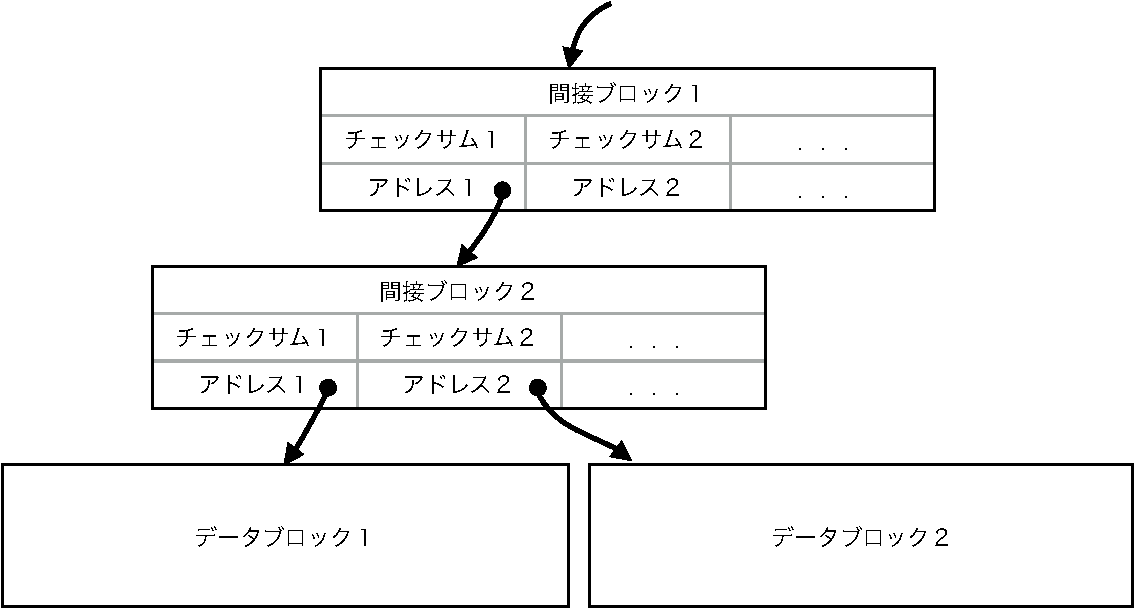
\includegraphics[scale=0.6]{Fig/zfsCheckSum-crop.pdf}}
  \end{myfig}

\item \emph{スナップショット}\footnote{
    ある時点のファイルシステムをコピーして凍結したもの.
    変更ができない.
  }や\emph{クローン}\footnote{
    ある時点のファイルシステムをコピーしたもの.
    変更ができる.
  }の作成は,
  \figref{zfsCheckSum}において最上位のブロックのコピーを作るような作業である.
  一瞬で作成が完了する.
  その後は COW の手法を使用し,
  コピーとオリジナルに違いが出た時点で,
  違いが出たブロックとそれの親だけのコピーが作られる.
  デバイスの容量も無駄にならない.

\item ボリュームの代わりにストレージプールと呼ばれる
  ソフトウェアの層をデバイスとファイルシステムの間にはさんでいる.
  従来のボリュームを模式的に表したものを\figref{zfsVolume}に,
  ZFSのストレージプールを模式的に表したものを\figref{zfsPool}に示す.

  \begin{myfig}{btp}{従来のボリューム}{zfsVolume}
    \centering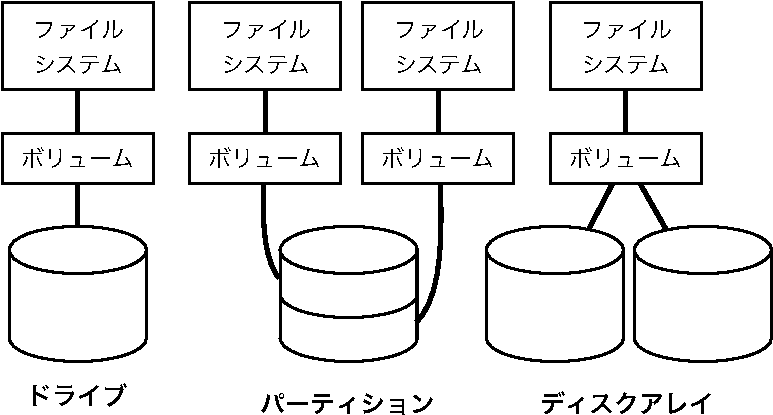
\includegraphics[scale=0.65]{Fig/zfsVolume-crop.pdf}
  \end{myfig}

  \begin{myfig}{btp}{ストレージプール}{zfsPool}
    \centering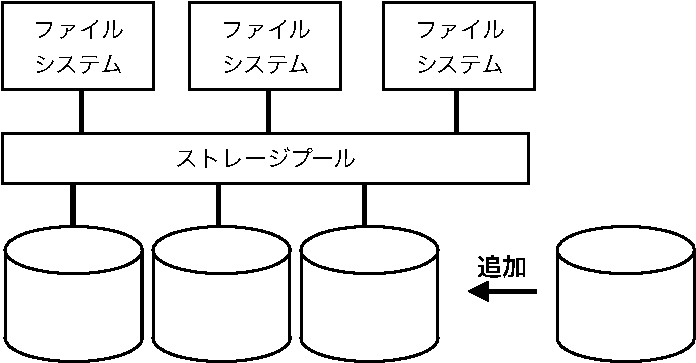
\includegraphics[scale=0.65]{Fig/zfsPool-crop.pdf}
  \end{myfig}
  
  従来は,ファイルシステムの初期化以前にボリュームを決定し,
  後で変更することはできなかった.
  ZFSのストレージプールは沢山のデバイスを収容し,
  ZFSからの要求に応じてデータブロックを割り付ける.
  C言語プログラムが\|malloc()|や\|free()|を使用して
  必要な時にメモリを割当てる方式に似ている.
  また,ストレージプールには後でデバイスを
  追加することも可能である.

\item ファイルサイズ等の制約が事実上無くなった.
  ファイルサイズは最大$2^{64}$バイト,
  ストレージプールサイズは最大$2^{70}$バイト\footnote{
    $Zetta = 2^{70}$ がZFSの名前に関係しているらしい.
  }である.

\item ストレージプールは,
  ミラーやRAID-Z\footnote{
    RAID-5の変形版のことである.
  }\cite{RaidzOfFreeBSD}等によりデバイスの故障に対する信頼性・可用性を向上する
  仕組みを持っている.

\item ストレージプールは,
  データ圧縮や重複除去の機能を持っている.
  データを圧縮することで読み書きするデータの量が減少するので,
  ファイルの読み書き性能が高くなることもある\footnote{
    ディスクに比較するとCPUはとても速い.}.
\end{itemize}

逆に,弱点としては次が挙げられる.
\begin{itemize}
\item 仮想記憶のページキャッシュと統合されていない.
\item CPUやメモリの利用率が高い.
  64ビットCPUでないとZFSに十分なメモリを提供できない.
\end{itemize}

%============================================================================
\section{ZFSのソフトウエア構成}
\figref{zfsSoftModule}にZFSを構成する主要なソフトウェアモジュールの関係を,
\figref{zfsTranscation}に
ソフトウェアモジュール間をデータが受け渡される様子を示す.
次にシステムコールが処理される手順を説明する.

\begin{myfig}{btp}{ZFSのソフトウェアモジュール}{zfsSoftModule}
  \centering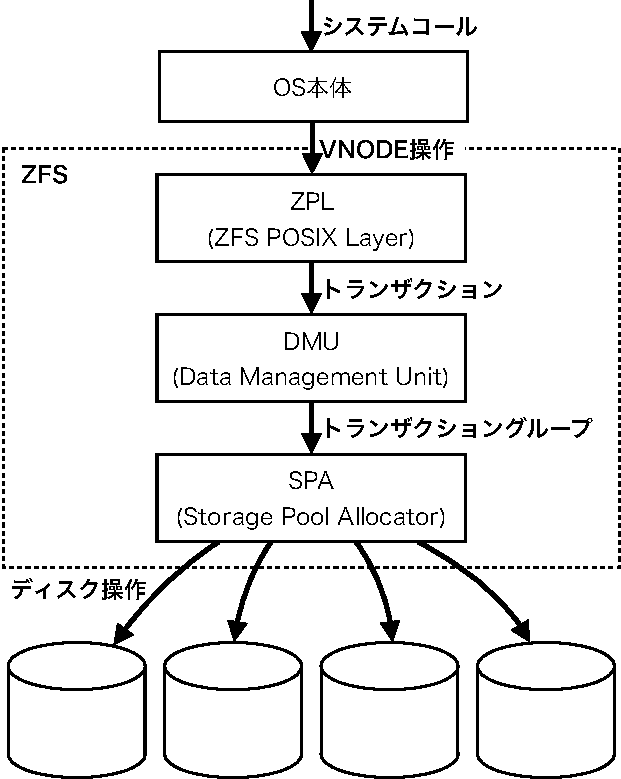
\includegraphics[scale=0.65]{Fig/zfsSoftModule-crop.pdf}
\end{myfig}
  
\begin{myfig}{btp}{トランザクションが書き込まれるまで}{zfsTranscation}
  \centering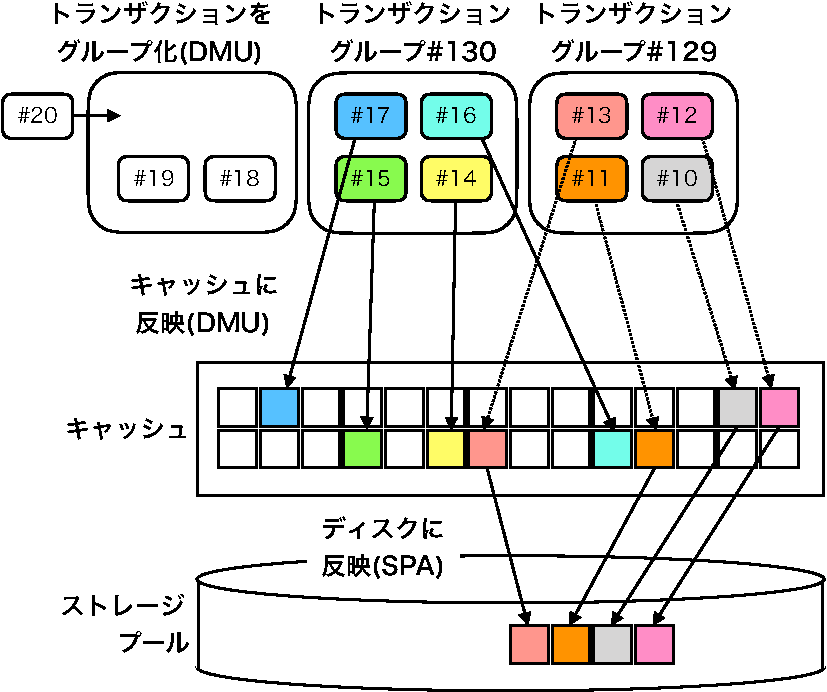
\includegraphics[scale=0.65]{Fig/zfsTranscation-crop.pdf}
\end{myfig}
  
\begin{enumerate}
\item アプリケーションが発行したシステムコールは,
  OSカーネル本体に含まれる上位ファイルシステムによりVNODE操作に変換される.
  VNODE操作は UNIX ファイルシステムの\inode の操作を仮想化したものである.
  VNODEインタフェースはZFS以前から用いられてきたものである.
  このインタフェースを用いてZFSのソフトウェアモジュールがOSに接続される.
  %VNODE操作を,
  %UNIXファイルシステムの操作に変換するソフトウェアモジュールを組合せたり,
  %FATファイルシステムに反映させるソフトウェアモジュールを組合せたりして
  %使用する.

\item ZPL(ZFS POSIX Layer)は VNODE 操作をZFSのトランザクションに変換する.
  1つのシステムコールが1つのトランザクションに変換される.

\item DMU(Data Management Unit)は複数のトランザクションをひとまとめにした
  \emph{トランザショングループ}を作る.
  DMUは,トランザクショングループ毎に,
  SPAが提供するストレージプールのキャッシュに書込みを行う.

\item SPA(Storage Pool Allocator)は,
  DMUがトランザクショングループをキャッシュに書込み終わると,
  キャッシュの内容をデバイスに反映させる.
  その際,なるべくデバイス上の連続セクタを使用するようにし,
  一度の書き込みで反映が終わるようにする\footnote{
    一度の書き込みで終わるほうが複数回の書き込みに分けるより速い.
    ホストコントローラがスキャッタギャザー(scatter gather)機能を
    持っていれば,
    メモリ上でバラバラに配置されたデータでも
    一度のコマンドで連続セクタにバースト書き込みすることができる.
  }.
\end{enumerate}

%============================================================================
\section{ストレージプールの構造(概要)}
ストレージプールは一般に複数のデバイスから構成されるが,
ここでは話を簡単にするために
一台のデバイスだけでストレージプールが構成される場合を考える.
\figref{zfsDevice}は,
ストレージプールを構成するデバイスの内部を示している.
256KiBのボリュームラベル(VL)が,
安全のためデバイス先頭に2箇所,末尾に2箇所,合計4箇所に記録されている.

ボリュームラベルの内部の構造は\figref{zfsVolumeLabel}のようになっている.
前半にはデバイスに関する情報(デバイスの名前など)が格納される.
後半は128個のUberblockを格納する配列である.
トランザクショングループがプールに書き込まれると,
最後にUberblockがトランザクショングループ番号とともに書き込まれる.
書き込まれる位置はトランザクショングループ番号を128で割った余りで計算できる.

\begin{figure}[btp]
  \centering
  \begin{minipage}{0.4\columnwidth}
    \centering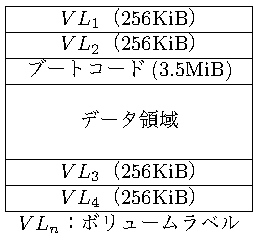
\includegraphics[scale=1.0]{Fig/zfsDevice.pdf}
    \caption{デバイス内部の配置}
    \label{fig:zfsDevice}
  \end{minipage}
  \begin{minipage}{0.4\columnwidth}
    \centering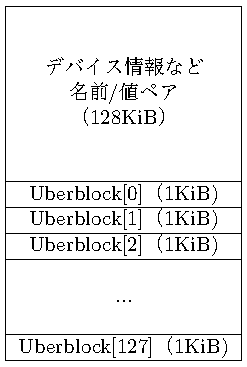
\includegraphics[scale=1.0]{Fig/zfsVolumeLabel.pdf}
    \caption{ボリュームラベルの内容}
    \label{fig:zfsVolumeLabel}
  \end{minipage}
\end{figure}

クラッシュや突然の停電により
システムが正常にシャットダウンされなかった場合でも,
全てのボリュームラベルのUberblock配列から,
トランザクショングループ番号を手がかりに最も新しいUberblockを見つけ出せば,
最後に書き込みが完了した時点のストレージプールの状態を再現できる.


%============================================================================
\section{ストレージプールの更新}
既に\figref{zfsCheckSum}に示したような\footnote{
  \figref{zfsCheckSum}はファイルのデータブロックを管理している
  様子である.ストレージプール全体ではもっと複雑になる.
}木構造を用いてメタデータブロックやデータブロックが記録される.
この木構造はストレージプールに記録される.
木構造のルートの位置はUberblockに記録される.
トランザクショングループの操作がストレージプールに反映される
様子を\figref{zfsCommit}に模式的に示す.

\begin{myfig}{btp}{ストレージプールのCOWによる更新のイメージ図}{zfsCommit}
  \centering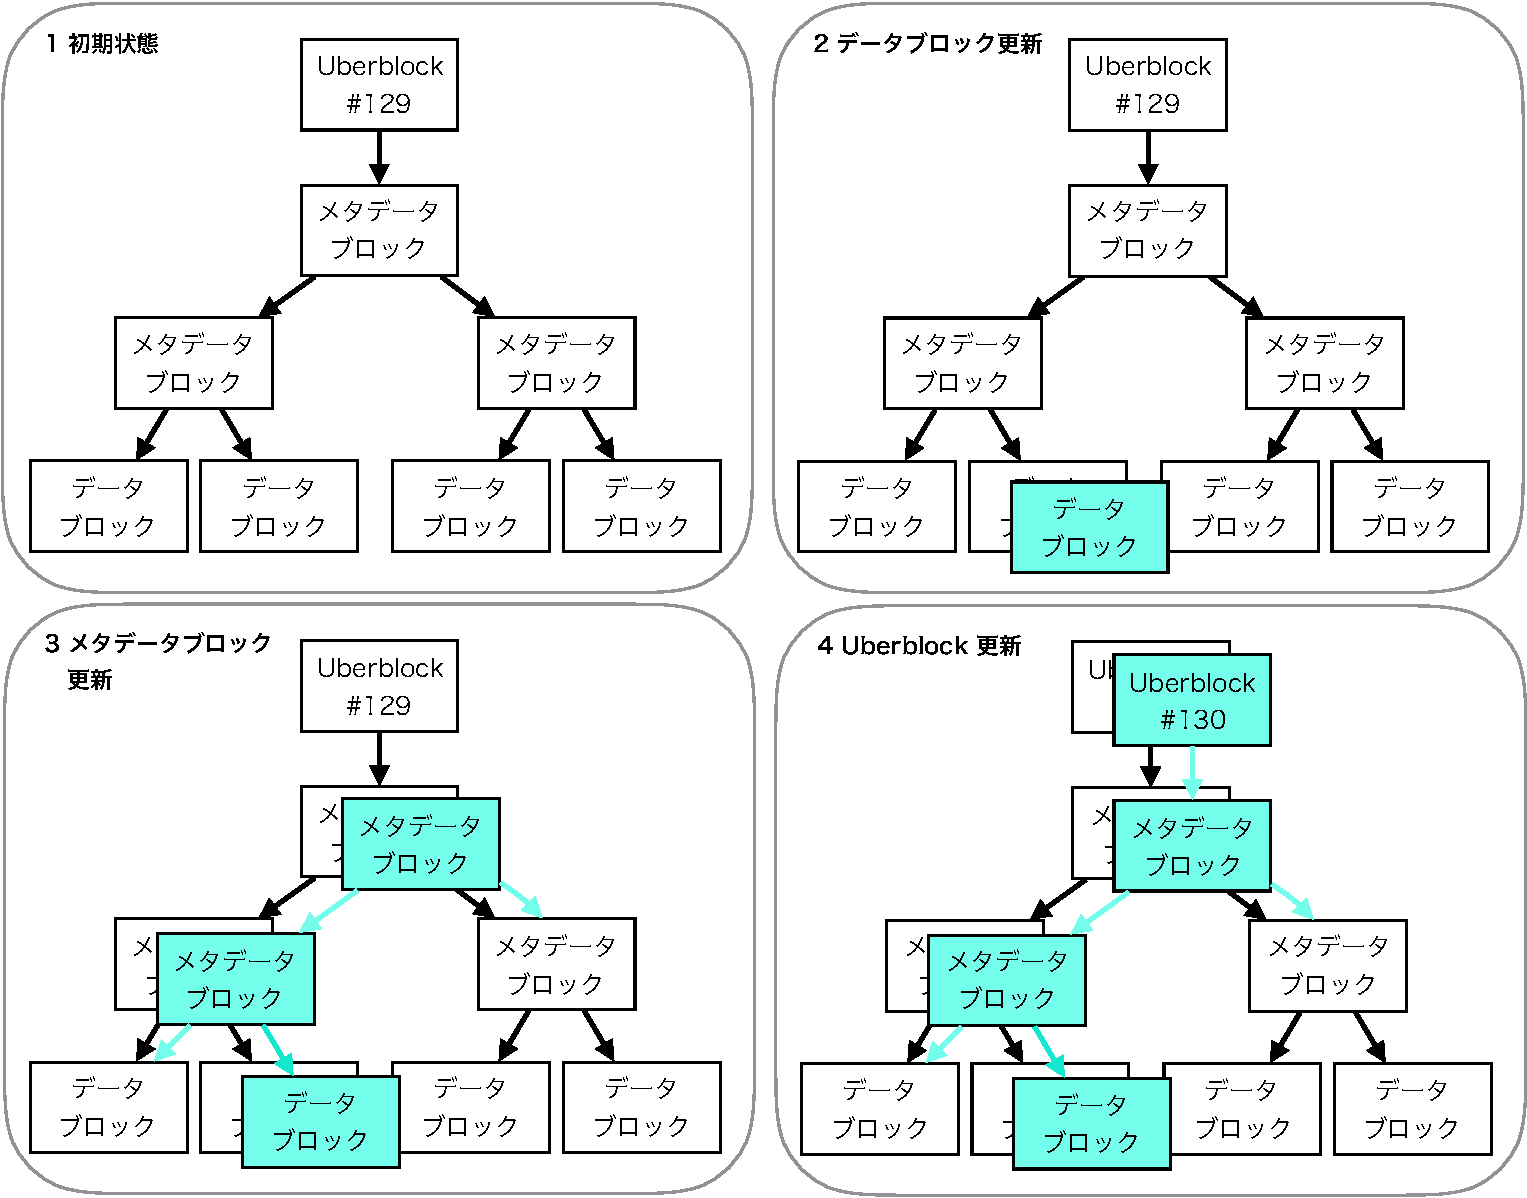
\includegraphics[scale=0.6]{Fig/zfsCommit-crop.pdf}
\end{myfig}

\begin{enumerate}
\item \emph{初期状態} \\
  デバイス上のストレージプールには,
  Uberblockを起点にする木構造でストレージプールのメタデータブロックや
  データブロックが記録されている.
\item \emph{データブロック更新} \\
  ストレージプールのデータブロックに変更あった場合,
  そのブロックを上書きするのでは無く,
  別のブロックを確保し新しい内容をそこに書き込む(COW).
\item \emph{メタデータブロック更新} \\
  変更のあったブロックを指すメタデータブロック中のポインタは,
  新しいブロックを指すように変更されなけばならない.
  別に新しいブロックを確保し,
  ポインタを更新した新しい内容をそこに書き込む(COW).
  この作業を木構造のルートまで繰り返す.
\item \emph{Uberblock更新} \\
  木構造の新しいルートを指すようにUberblockを変更する.
  この際も,既存のUberblockを上書きするのではなく,
  新しいUberblockを使用する.
  Uberblockにトランザクショングループ番号を書き込むことで,
  どのUberblockが最新のものか区別できるようになっている.
  トランザクショングループ番号は64ビットなので,
  システムが廃棄されるまでオーバーフローする心配はない.
\end{enumerate}

以上の手順では,
Uberblockが正常に更新されるまで新しいデータは全く反映されない.
どの段階でシステムがクラッシュしても,
ストレージプールの状態はトランザクションが適用される前か,
トランザクションが完了した後のどちらかになる.

Uberblockが正常に更新されどこからも指されなくなったブロックは再利用される.

%============================================================================
\section{ストレージプールの構造}

\subsection{ブロックポインタ}
\figref{zfsCheckSum}で,「チェックサム」,「アドレス」と表現した部分は
\emph{ブロックポインタ}と呼ばれる128バイトのデータである.
ブロックポインタはデータ多重化のために最大3組のアドレスを記録できる.
%以下では1組だけ使用する場合を説明する.
ブロックポインタには以下の情報が含まれる.
\begin{itemize}
\item \emph{サイズ}:ブロックの大きさに関する情報である.
\item \emph{チェックサム}(256ビット):ブロックのチェックサムである.
\item \emph{ブロックのアドレス}:
  ブロックのストレージプール内での格納位置に関する情報である.(最大3個)
\item \emph{タイムスタンプ}:
  ブロックを作成したトランザクショングループの番号である.
  ファイルシステムからブロックが削除される時,
  ファイルシステムのスナップショットのタイムスタンプと比較する.
  スナップショットより古いブロックはスナップショットで使用されているので,
  削除できない.
\item \emph{その他}:チェックサム計算に使用するアルゴリズムの種類,
  データ圧縮に使用するアルゴリズムの種類,圧縮後のサイズなど,
  ここでは紹介しない情報が含まれる.
\end{itemize}

\subsection{Dnode}
\emph{dnode}はストレージプール内の
あらゆるオブジェクトを表現する512バイトのデータ構造である.
UFSの{\inode}に似ているがdnodeはファイルやディレクトリだけでなく,
ファイルシステムや,スナップショット,クローンなどの表現にも用いられる.
dnodeは表現するオブジェクトや,
付属するデータの大きさによって幾つかの形式を取るが,
ファイルを表現する場合の例を\figref{zfsDnode}に示す.

\begin{myfig}{btp}{ファイルを表現するdnodeの例}{zfsDnode}
  \centering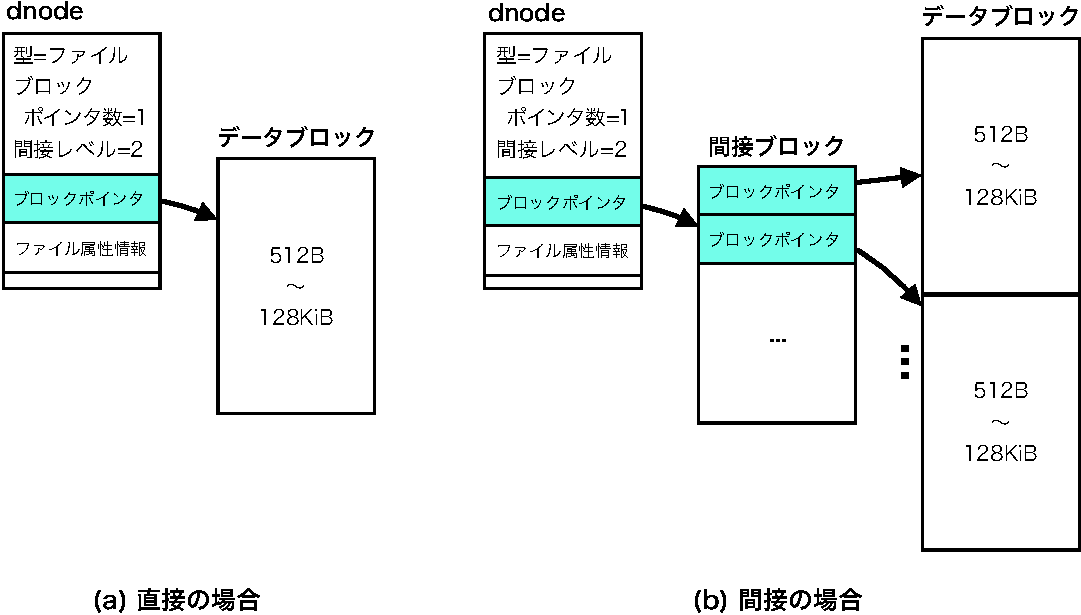
\includegraphics[scale=0.75]{Fig/zfsDnode-crop.pdf}
\end{myfig}

以下では,\figref{zfsDnode}について説明する.
\figref{zfsDnode}はファイルを表現するdnodeの例であるが,
ファイル以外のオブジェクトも同様な方法でデータを格納する.

\begin{itemize}
\item dnodeは三つ以内のブロックポインタを格納することができる.
  図は一つのブロックポインタを格納した例である.
\item dnodeは表現するオブジェクトに応じたデータを格納する領域を持っている.
  この領域はブロックポインタと共用になっているので,
  ブロックポインタの数が多い場合は小さくなる.
  図の例はdnodeがファイルを表現する場合なので,
  ファイルの属性情報(時刻や保護属性など)を格納している.
\item データの大きさが128KiB以内の場合は,図の(a)に示すように
  dnodeのブロックポインタがデータブロックを直接参照する.
\item 大きさが128KiBを超える場合は,
  図の(b)に示すようにdnodeのブロックポインタが間接ブロックを指すようになる.
  最大128KiBの間接ブロックは128Bのブロックポインタを最大1Ki個格納できる.
\item $128KiB \times 1Ki = 128MiB$より大きなデーを表現する時は,
  UFSのように多重の間接ブロックを用いる.
  間接レベルは6までサポートされており,
  $2^{64}$バイト以上のファイルが表現できる.
  UFSではファイルの後方のデータブロックだけが間接ブロックになったが,
  すべてのブロックが同じ間接レベルで扱われる.
\end{itemize}

\subsection{全体像}
\figref{zfsStructure}にストレージプールの構造を
模式的に描いたものを示す.
Objsetはdnodeの配列を管理する2KiB\footnote{
\url{https://people.freebsd.org/~gibbs/zfs_doxygenation/html/annotated.html}
に公開されているFreeBSD ZFSの実装を前提にしている.
}のデータ構造である.
Objsetに埋め込まれたdnodeが,dnode配列を格納するブロックを管理する.
Objsetには最大三つのdnodeを埋め込むことができる.

\begin{myfig}{btp}{ストレージプールの構造}{zfsStructure}
  \centering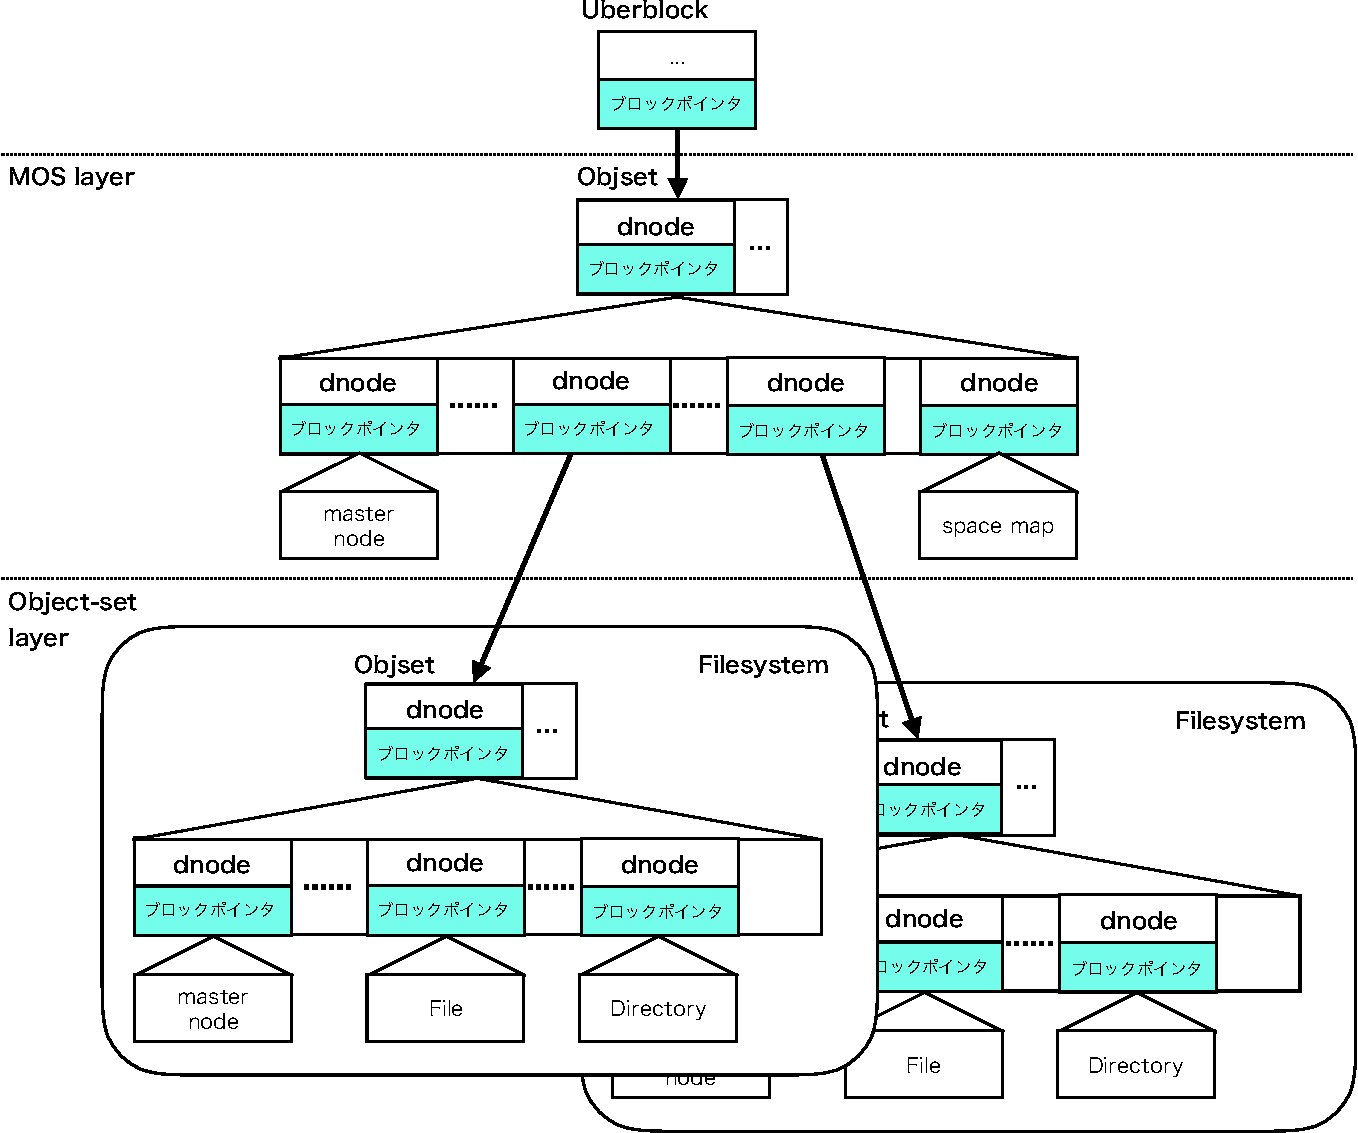
\includegraphics[scale=0.7]{Fig/zfsStructure-crop.pdf}
\end{myfig}

\subsubsection{MOS(Meta Object Set) layer}
\emph{MOS layer}はストレージプール全体に関わるオブジェクトや,
ファイルシステムやスナップショット,クローンなどの根になるdnodeを格納する.
オブジェクトの種類はdnodeの型から分かる.
\begin{itemize}
\item dnode配列の先頭は\emph{master node}である.
  master node はストレージプールのコンフィグ,プロパティ,
  エラーログ,統計情報などを記録する.
\item dnode配列の最後には\emph{space map}が格納される.
  space map はストレージプール内のブロックの割付を管理する.
\item dnode配列の他の要素は,
  Object-set layerのファイルシステムやスナップショット,
  クローンなどの根になるdnodeを格納する.
\end{itemize}

\subsubsection{Object-set layer}
\emph{Object-set layer}はファイルシステムやスナップショット,
クローンなどの実体を格納する.
\figref{zfsStructure}では二つのファイルシステムがObject-set layerに
格納されている様子を表している.

\begin{itemize}
\item ファイルシステムはObjsetが管理するdnodeリストにより表現される.
\item このdnodeリストがUFSの{\inode}リストに相当する.
\item dnodeリスト先頭の master node は root ディレクトリの dnode 番号や
  ファイルシステムのバージョン番号などを格納している.
\item dnodeリストの二番目の dnode は通常ファイルを表現している.
\item dnodeリストの三番目の dnode はディレクトリファイルを表現している.
  ディレクトリファイルは\emph{ファイル名とdnode番号の対応表}である.
\item 図ではObjsetはファイルシステム本体だけ管理しているが,
  実際はユーザやグループ毎の記憶領域の使用量を管理するオブジェクトや,
  ファイルシステムでは使用されなくなったが
  スナップショットが使用しているために解放できないブロックの
  リスト(deadlist)なども管理している.
\end{itemize}

%============================================================================
\section{スナップショットとクローン}
ある時点のファイルシステムの状態をコピーして凍結したものを
\emph{スナップショット}と呼ぶ.
スナップショットをもとに変更可能にしたものを\emph{クローン}と呼ぶ.

\subsection{スナップショットの作成}
\figref{zfsSnapshot}は
ZFSがスナップショットやクローンを作る原理を説明している.
スナップショットの作成は次の二つのステップでできる.

\begin{myfig}{btp}{スナップショットの作成}{zfsSnapshot}
  \centering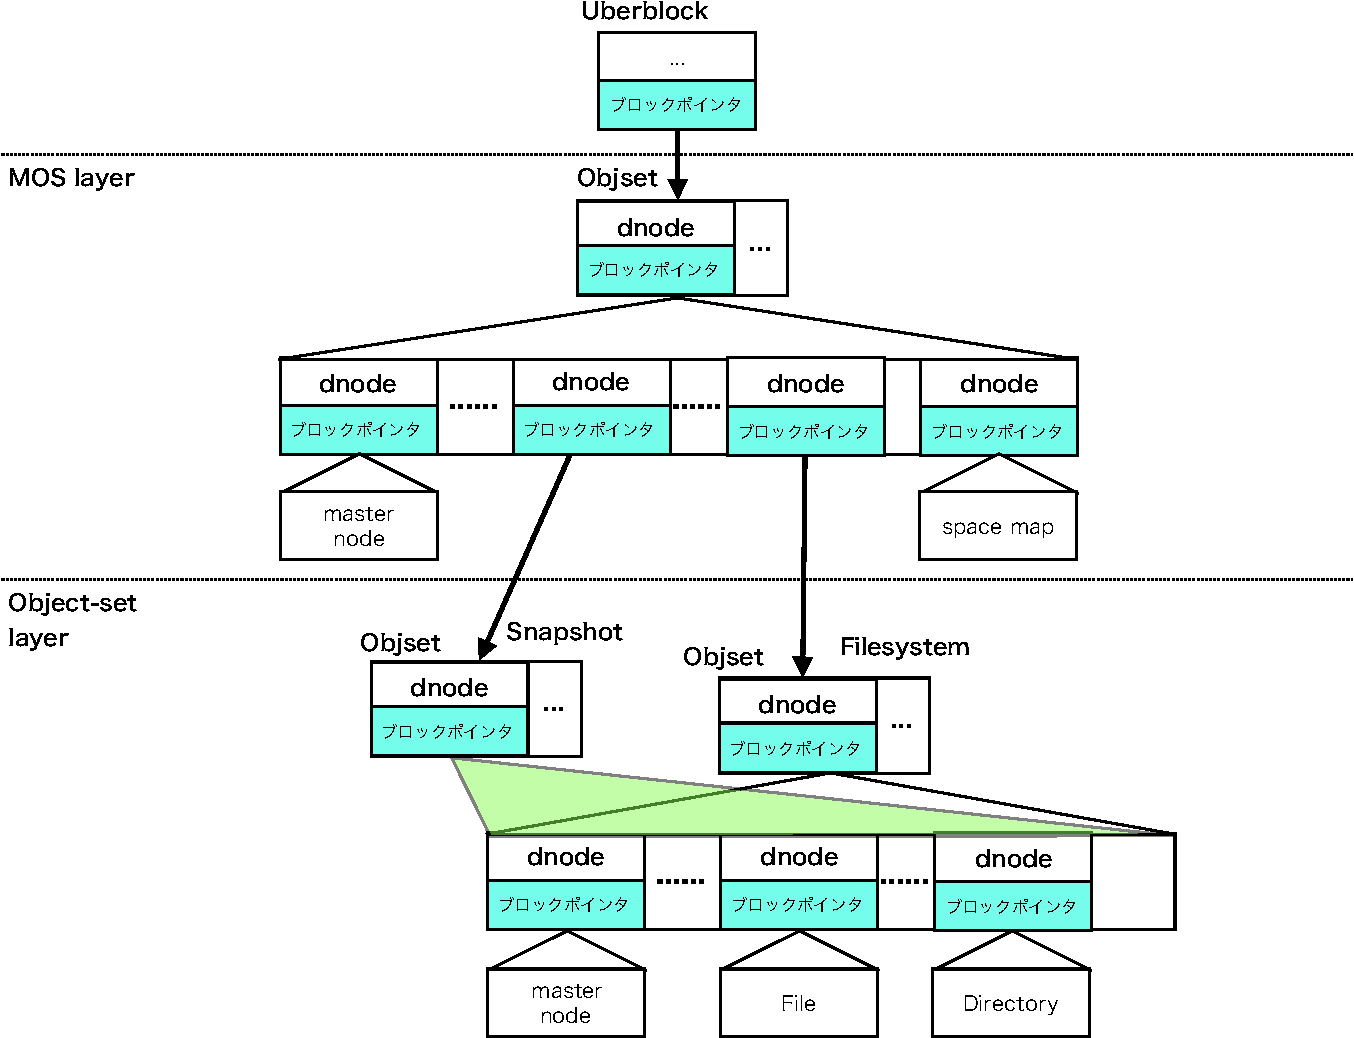
\includegraphics[scale=0.7]{Fig/zfsSnapshot-crop.pdf}
\end{myfig}

\begin{enumerate}
\item Object-set layerに格納されているファイルシステムのObjsetのコピーを作る.
\item MOS layer の dnode 配列に新しい dnode を追加し,
  Objsetのコピーを参照するようにする.
\end{enumerate}

スナップショットの作成は一瞬で完了する.
スナップショットは読み出し専用なのでObjset以下は変化しない.
しかし,ファイルシステムは変化する.
ファイルシステムが変化した時はCOWを用いて必要最小限の範囲の
ブロックだけ書き換える.

\subsection{ブロックの解放}
通常,
COWにより新しいコピーに役割を譲ったストレージプールのブロックは解放される.
しかし,スナップショットがある場合,
ブロックがスナップショットからも参照されている可能性があるので
解放しても良いか判断が難しくなる.
そこで,ブロックポインタにリンクカウントを設ける方法が考えられる.
しかし,この方法ではスナップショットを作るたびに
ファイルシステムの全てのブロックポインタを書き換える必要が生じる.

\subsubsection{スナップショットとdeadlistの構造}
ZFSではブロックポインタのタイムスタンプとスナップショットのタイムスタンプを
比較することで,解放しても良いブロックかどうか判断している.
そのために MOS layerで,同じファイルシステムから過去に作成した
スナップショットがどれか分かるように管理している.
タイムスタンプには,現実の時刻ではなく,
トランザクショングループ番号が用いられる.
また,ファイルシステムのObjsetは,
現在は使用していないがスナップショットで使用されていないため解放できない
ブロックのリスト(deadlist)も管理している.
その様子を\figref{zfsDeadlist1}に示す.

\begin{myfig}{btp}{スナップショットとdeadlist}{zfsDeadlist1}
  \centering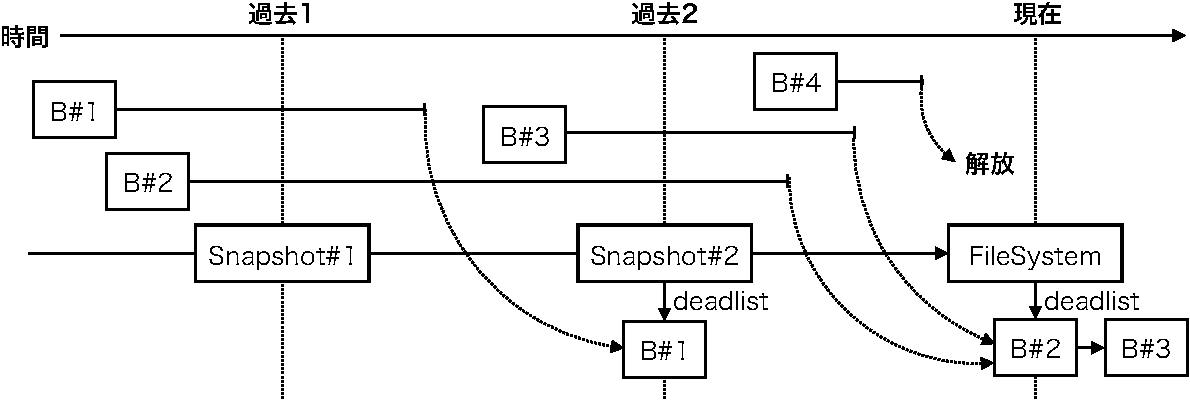
\includegraphics[scale=0.7]{Fig/zfsDeadlist1-crop.pdf}
\end{myfig}

\begin{itemize}
\item \|B#N|はブロックを表している.
  ブロックを指すブロックポインタが,タイムスタンプを格納する.
  ブロックから右に伸びる直線は,
  ブロックが割り当てられてから
  ファイルシステムで使用されなくなるまでの時間を表している.
\item \|Snapshot#N|はスナップショットを表している.
  図では,「過去1」,「過去2」の二回スナップショットが作成されている.
  スナップショット作成時点では使用されていなかったが,
  過去のスナップショットから参照されているため解放できないブロックのリスト
  である\|deadlist|を持っている.
\item \|FileSystem|は現在アクティブなファイルシステムを表している.
  現在は使用されていないがスナップショットから参照されている
  ブロックのリストである\|deadlist|を持っている.
\end{itemize}

\subsubsection{使用されなくなったブロック}
\figref{zfsDeadlist1}は,
「過去1」から「現在」までの間に\|B#1|,\|B#2|,\|B#3|,\|B#4|の
四つのブロックが使用されなくなった場合を説明してる.

\begin{itemize}
\item \|B#1|は\|Snapshot#1|と\|Snapshot#2|の間で使用されなくなったが,
  \|Snapshot#1|よりも前から使用されていた.
  \|Snapshot#1|で使用されているので解放できない.
  その時点でアクティブな\|FileSystem|の\|deadlist|に入れる.
  \|Snapshot#2|作成時に\|deadlist|はスナップショット側に残される.
  \|FileSystem|の\|deadlist|は空になる.
\item \|B#2|と\|B#3|は\|Snapshot#2|より前に割り当てられていた.
  これらのブロックは過去のスナップショットで使用されているので,
  現在のファイルシステムで使用されなくなっても解放できない.
  \|FileSystem|の\|deadlist|に入れる.
\item \|B#4|は\|Snapshot#2|(最新のスナップショット)より後に割り当てられ,
  短時間の内に使用されなくなったブロックである.
  このブロックは,どのスナップショットでも使用されていないので解放できる.
\end{itemize}

\subsubsection{スナップショットの削除}
\figref{zfsDeadlist1}から\|Snapshot#2|を削除したものを
\figref{zfsDeadlist2}に示す.
以下では\|Snapshot#2|を削除する手順を説明する.
\|Snapshot#2|が削除されると最新のスナップショットが\|Snapshot#1|になるので,
それに応じた処理が必要になる.

\begin{myfig}{btp}{スナップショットの削除}{zfsDeadlist2}
  \centering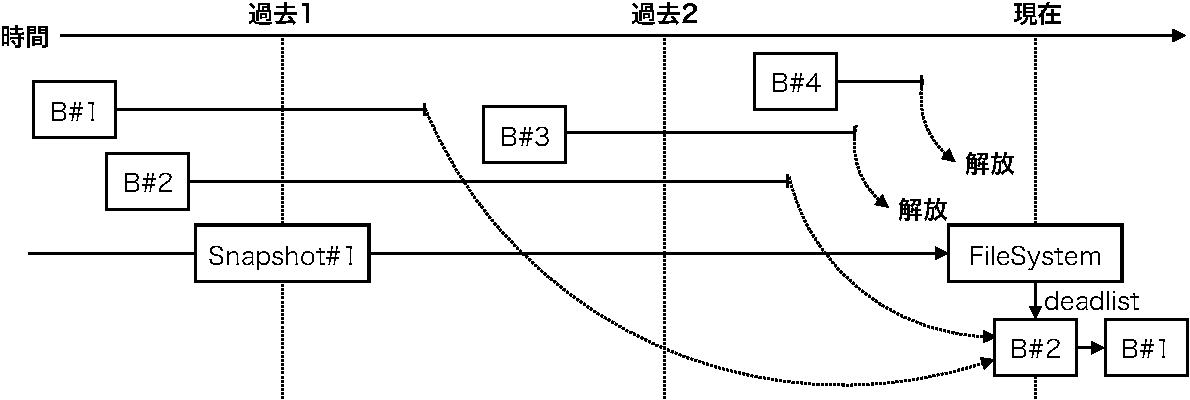
\includegraphics[scale=0.7]{Fig/zfsDeadlist2-crop.pdf}
\end{myfig}

\begin{itemize}
\item \|FileSystem|の\|deadlist|にあった\|B#3|は,
  最新のスナップショットが\|Snapshot#1|になったので,
  開放することができる.
\item \|Snapshot#2|の\|deadlist|にあった\|B#1|は,
  \|Snapshot#1|より前に割り当てられたものなので解放できない.
  \|FileSystem|の\|deadlist|に移動する.
\end{itemize}

%============================================================================
\section{まとめ}
ZFSは大きな主記憶と高速なCPUを前提に設計された新しいファイルシステムである.
以下のような多くの特徴を持っている.
\begin{itemize}
\item COW(Copy On Write)を用い既存のブロックを上書きすることがない.
\item COWを活用し,システムが突然に停止するような事態があっても,
  ファイルシステムが壊れない構造を実現している.
\item デバイス上の全てのデータについてチェックサムを持ち,
  高い信頼性を確保している.
\item ファイルシステム全体のコピーであるスナップショットやクローンを
  一瞬で作ることができる.
\item ボリュームの代わりにストレージプールを使用する.
  ストレージプールには後で新しいデバイスを追加することもできる.
\end{itemize}

本章では,ZFSを管理する主要なソフトウェアモジュール,
ストレージプールの構造や更新手順,
ファイルシステムを格納したストレージプール全体像,
スナップショットやクローンの仕組みについて紹介した.

%==============================================================================
\newpage
\section*{練習問題}
\begin{enumerate}
  \renewcommand{\labelenumi}{\ttfamily\arabic{chapter}.\arabic{enumi}}
  \setlength{\leftskip}{1em}
\item 次の言葉の意味を説明しなさい.
  また,分からない言葉について調べなさい.
  \begin{itemize}
  \item COW(Copy On Write)
  \item メタデータ
  \item チェックサム
  \item スナップショット
  \item クローン
  \item ボリューム
  \item ストレージプール
  \item ZPL(ZFS POSIX Layer)
  \item DMU(Data Management Unit)
  \item SPA(Storage Pool Allocator)
  \item VNODE
  \item Uberblock
  \item ブロックポインタ
  \item Dnode
  \item MOS(Meta Object Set) layer
  \item Object-set layer
  \item space map
  \item master node
  \end{itemize}
  \item トランザクショングループ番号は64ビットです.
    毎秒100トランザクショングループを処理したとして,
    トランザクショングループ番号がオーバーフローするまでに約何年かかるか
    計算しなさい.
  \item ZFSで使用できるチェックサム計算アルゴリズムについて調べなさい.
  \item ファイルを表現するdnodeが間接レベル2の時,
    最大のファイルサイズは何バイトになるか計算しなさい.
  \item ブロックにリンクカウントを設け,
    スナップショットからの参照数を管理することで,
    ブロックの解放を判断するアイデアの利点と問題点を挙げなさい.
\end{enumerate}
